% Options for packages loaded elsewhere
\PassOptionsToPackage{unicode}{hyperref}
\PassOptionsToPackage{hyphens}{url}
%
\documentclass[
]{book}
\title{La tarification a priori}
\author{Abdoul Oudouss DIAKITE, Othmane ETTADLAOUI}
\date{}

\usepackage{amsmath,amssymb}
\usepackage{lmodern}
\usepackage{iftex}
\ifPDFTeX
  \usepackage[T1]{fontenc}
  \usepackage[utf8]{inputenc}
  \usepackage{textcomp} % provide euro and other symbols
\else % if luatex or xetex
  \usepackage{unicode-math}
  \defaultfontfeatures{Scale=MatchLowercase}
  \defaultfontfeatures[\rmfamily]{Ligatures=TeX,Scale=1}
\fi
% Use upquote if available, for straight quotes in verbatim environments
\IfFileExists{upquote.sty}{\usepackage{upquote}}{}
\IfFileExists{microtype.sty}{% use microtype if available
  \usepackage[]{microtype}
  \UseMicrotypeSet[protrusion]{basicmath} % disable protrusion for tt fonts
}{}
\makeatletter
\@ifundefined{KOMAClassName}{% if non-KOMA class
  \IfFileExists{parskip.sty}{%
    \usepackage{parskip}
  }{% else
    \setlength{\parindent}{0pt}
    \setlength{\parskip}{6pt plus 2pt minus 1pt}}
}{% if KOMA class
  \KOMAoptions{parskip=half}}
\makeatother
\usepackage{xcolor}
\IfFileExists{xurl.sty}{\usepackage{xurl}}{} % add URL line breaks if available
\IfFileExists{bookmark.sty}{\usepackage{bookmark}}{\usepackage{hyperref}}
\hypersetup{
  pdftitle={La tarification a priori},
  pdfauthor={Abdoul Oudouss DIAKITE, Othmane ETTADLAOUI},
  hidelinks,
  pdfcreator={LaTeX via pandoc}}
\urlstyle{same} % disable monospaced font for URLs
\usepackage{color}
\usepackage{fancyvrb}
\newcommand{\VerbBar}{|}
\newcommand{\VERB}{\Verb[commandchars=\\\{\}]}
\DefineVerbatimEnvironment{Highlighting}{Verbatim}{commandchars=\\\{\}}
% Add ',fontsize=\small' for more characters per line
\usepackage{framed}
\definecolor{shadecolor}{RGB}{248,248,248}
\newenvironment{Shaded}{\begin{snugshade}}{\end{snugshade}}
\newcommand{\AlertTok}[1]{\textcolor[rgb]{0.94,0.16,0.16}{#1}}
\newcommand{\AnnotationTok}[1]{\textcolor[rgb]{0.56,0.35,0.01}{\textbf{\textit{#1}}}}
\newcommand{\AttributeTok}[1]{\textcolor[rgb]{0.77,0.63,0.00}{#1}}
\newcommand{\BaseNTok}[1]{\textcolor[rgb]{0.00,0.00,0.81}{#1}}
\newcommand{\BuiltInTok}[1]{#1}
\newcommand{\CharTok}[1]{\textcolor[rgb]{0.31,0.60,0.02}{#1}}
\newcommand{\CommentTok}[1]{\textcolor[rgb]{0.56,0.35,0.01}{\textit{#1}}}
\newcommand{\CommentVarTok}[1]{\textcolor[rgb]{0.56,0.35,0.01}{\textbf{\textit{#1}}}}
\newcommand{\ConstantTok}[1]{\textcolor[rgb]{0.00,0.00,0.00}{#1}}
\newcommand{\ControlFlowTok}[1]{\textcolor[rgb]{0.13,0.29,0.53}{\textbf{#1}}}
\newcommand{\DataTypeTok}[1]{\textcolor[rgb]{0.13,0.29,0.53}{#1}}
\newcommand{\DecValTok}[1]{\textcolor[rgb]{0.00,0.00,0.81}{#1}}
\newcommand{\DocumentationTok}[1]{\textcolor[rgb]{0.56,0.35,0.01}{\textbf{\textit{#1}}}}
\newcommand{\ErrorTok}[1]{\textcolor[rgb]{0.64,0.00,0.00}{\textbf{#1}}}
\newcommand{\ExtensionTok}[1]{#1}
\newcommand{\FloatTok}[1]{\textcolor[rgb]{0.00,0.00,0.81}{#1}}
\newcommand{\FunctionTok}[1]{\textcolor[rgb]{0.00,0.00,0.00}{#1}}
\newcommand{\ImportTok}[1]{#1}
\newcommand{\InformationTok}[1]{\textcolor[rgb]{0.56,0.35,0.01}{\textbf{\textit{#1}}}}
\newcommand{\KeywordTok}[1]{\textcolor[rgb]{0.13,0.29,0.53}{\textbf{#1}}}
\newcommand{\NormalTok}[1]{#1}
\newcommand{\OperatorTok}[1]{\textcolor[rgb]{0.81,0.36,0.00}{\textbf{#1}}}
\newcommand{\OtherTok}[1]{\textcolor[rgb]{0.56,0.35,0.01}{#1}}
\newcommand{\PreprocessorTok}[1]{\textcolor[rgb]{0.56,0.35,0.01}{\textit{#1}}}
\newcommand{\RegionMarkerTok}[1]{#1}
\newcommand{\SpecialCharTok}[1]{\textcolor[rgb]{0.00,0.00,0.00}{#1}}
\newcommand{\SpecialStringTok}[1]{\textcolor[rgb]{0.31,0.60,0.02}{#1}}
\newcommand{\StringTok}[1]{\textcolor[rgb]{0.31,0.60,0.02}{#1}}
\newcommand{\VariableTok}[1]{\textcolor[rgb]{0.00,0.00,0.00}{#1}}
\newcommand{\VerbatimStringTok}[1]{\textcolor[rgb]{0.31,0.60,0.02}{#1}}
\newcommand{\WarningTok}[1]{\textcolor[rgb]{0.56,0.35,0.01}{\textbf{\textit{#1}}}}
\usepackage{longtable,booktabs,array}
\usepackage{calc} % for calculating minipage widths
% Correct order of tables after \paragraph or \subparagraph
\usepackage{etoolbox}
\makeatletter
\patchcmd\longtable{\par}{\if@noskipsec\mbox{}\fi\par}{}{}
\makeatother
% Allow footnotes in longtable head/foot
\IfFileExists{footnotehyper.sty}{\usepackage{footnotehyper}}{\usepackage{footnote}}
\makesavenoteenv{longtable}
\usepackage{graphicx}
\makeatletter
\def\maxwidth{\ifdim\Gin@nat@width>\linewidth\linewidth\else\Gin@nat@width\fi}
\def\maxheight{\ifdim\Gin@nat@height>\textheight\textheight\else\Gin@nat@height\fi}
\makeatother
% Scale images if necessary, so that they will not overflow the page
% margins by default, and it is still possible to overwrite the defaults
% using explicit options in \includegraphics[width, height, ...]{}
\setkeys{Gin}{width=\maxwidth,height=\maxheight,keepaspectratio}
% Set default figure placement to htbp
\makeatletter
\def\fps@figure{htbp}
\makeatother
\setlength{\emergencystretch}{3em} % prevent overfull lines
\providecommand{\tightlist}{%
  \setlength{\itemsep}{0pt}\setlength{\parskip}{0pt}}
\setcounter{secnumdepth}{5}
\usepackage{booktabs}
\ifLuaTeX
  \usepackage{selnolig}  % disable illegal ligatures
\fi
\usepackage[]{natbib}
\bibliographystyle{apalike}

\usepackage{amsthm}
\newtheorem{theorem}{Theorem}[chapter]
\newtheorem{lemma}{Lemma}[chapter]
\newtheorem{corollary}{Corollary}[chapter]
\newtheorem{proposition}{Proposition}[chapter]
\newtheorem{conjecture}{Conjecture}[chapter]
\theoremstyle{definition}
\newtheorem{definition}{Definition}[chapter]
\theoremstyle{definition}
\newtheorem{example}{Example}[chapter]
\theoremstyle{definition}
\newtheorem{exercise}{Exercise}[chapter]
\theoremstyle{definition}
\newtheorem{hypothesis}{Hypothesis}[chapter]
\theoremstyle{remark}
\newtheorem*{remark}{Remark}
\newtheorem*{solution}{Solution}
\begin{document}
\maketitle

{
\setcounter{tocdepth}{1}
\tableofcontents
}
\hypertarget{introduction}{%
\chapter*{Introduction}\label{introduction}}
\addcontentsline{toc}{chapter}{Introduction}

L'assurance est une opération de risque d'un assuré à un assureur. Cette opération de transfert se fait par un paiement de prime par l'assuré à l'assureur. Ce dernier s'engage à indemniser son client en cas de survenance d'un sinistre pendant toute la période couverte par le contrat.
La prime reçue par l'assureur doit refléter le risque qu'il est prêt à couvrir d'où la nécessité de se demander combien faut-il recevoir en prime pour assurer \(\lambda\) niveau de risque ?

\hypertarget{objectif}{%
\section{Objectif}\label{objectif}}

Dans ce projet, nous allons faire une étude sur des données que nous décrirons plus tard. Le but est d'appliquer différentes méthodes vues en assurance non-vie et de ressortir le meilleur modèle de tarification. Bien sûr nous allons commencer par une étude statistique de nos données ainsi qu'un ensemble de représentations graphiques.

\hypertarget{les-donnuxe9es-du-projets}{%
\section{Les données du projets}\label{les-donnuxe9es-du-projets}}

Cette base de données contient 16082 images d'une assurance automobile. (\href{https://github.com/AODiakite/Tarification/blob/master/data/base5.sas7bdat}{\emph{Télécharger}}).
Le code suivant permet de charger les données qui se trouvaient au préalable dans le dossier \emph{Data}.

\begin{Shaded}
\begin{Highlighting}[]
\FunctionTok{library}\NormalTok{(haven)}
\NormalTok{database }\OtherTok{\textless{}{-}} \FunctionTok{read\_sas}\NormalTok{(}\StringTok{"Data/base5.sas7bdat"}\NormalTok{, }
    \ConstantTok{NULL}\NormalTok{)}
\NormalTok{knitr}\SpecialCharTok{::}\FunctionTok{kable}\NormalTok{(}
  \FunctionTok{head}\NormalTok{(database[,}\DecValTok{1}\SpecialCharTok{:}\DecValTok{8}\NormalTok{], }\DecValTok{10}\NormalTok{), }\AttributeTok{booktabs =} \ConstantTok{TRUE}\NormalTok{,}
  \AttributeTok{caption =} \StringTok{\textquotesingle{}A table of the first 10 rows of our data.\textquotesingle{}}
\NormalTok{)}
\end{Highlighting}
\end{Shaded}

\begin{table}

\caption{\label{tab:unnamed-chunk-1}A table of the first 10 rows of our data.}
\centering
\begin{tabular}[t]{rrllllrr}
\toprule
NAP & PERMIS & DEB\_IMAG & FIN\_IMAG & SEX & STATUT & CSP & USAGE\\
\midrule
83 & 332 & 2004-01-01 & 2004-02-01 & M & A & 50 & 3\\
916 & 333 & 2004-02-01 & NA & M & A & 50 & 3\\
550 & 173 & 2004-05-15 & 2004-12-03 & M & A & 50 & 2\\
89 & 364 & 2004-11-29 & NA & F & A & 55 & 2\\
233 & 426 & 2004-02-07 & 2004-05-01 & M & A & 60 & 1\\
\addlinespace
666 & 429 & 2004-05-01 & NA & M & A & 60 & 1\\
80 & 461 & 2004-04-02 & 2004-05-01 & M & A & 48 & 3\\
666 & 462 & 2004-05-01 & NA & M & A & 48 & 3\\
173 & 405 & 2004-10-29 & NA & F & A & 50 & 2\\
474 & 386 & 2004-01-01 & 2004-06-22 & M & A & 55 & 2\\
\bottomrule
\end{tabular}
\end{table}

\hypertarget{description-des-donnuxe9es}{%
\section{Description des données}\label{description-des-donnuxe9es}}

Évidemment, il est très difficile de comprendre certaines abréviations dans les données que nous venons de télécharger. Ne vous inquiétez surtout pas ! Le tableau suivant contient la \href{https://github.com/AODiakite/Tarification/blob/master/data/D\%C3\%A9tails\%20des\%20variables.xls}{description} de chaque colonne de la base 5 que nous appellerons dorénavant \textbf{\emph{database}}.

\begin{table}

\caption{\label{tab:unnamed-chunk-2}Descriptions de database.}
\centering
\begin{tabular}[t]{ll}
\toprule
Description & Code\\
\midrule
age du conducteur & agecond\\
ancienneté de permis & permis\\
sexe du conducteur & sex\\
statut matrimonial & statut\\
catégorie socio-professionnelle & csp\\
\addlinespace
usage du véhicule & usage\\
option kilométrage limité & k8000\\
zone géographique & zone\\
coefficient de réduction majoration (bonus/malus) & RM\\
date de début d'image & deb\_imag\\
\addlinespace
date de fin d'image & fin\_imag\\
nombre d'années-police & nap\\
nombre de sinistres responsables dans les 4 années précédent l'image & sinap1\\
nombre de sinistres non responsables dans les 4 années précédent l'image & sinap2\\
nombre de sinistres parking dans les 4 années précédent l'image & sinap3\\
\addlinespace
nombre de sinistres incendie/vol dans les 4 années précédent l'image & sinap4\\
nombre de sinistres bris de glace dans les 4 années précédent l'image & sinap5\\
nombre de mises en demeure dans les 4 années précédent l'image & sinap6\\
charge de sinistres & charge\\
\bottomrule
\end{tabular}
\end{table}

\begin{quote}
Passons maintenant à l'étude statistique !
\end{quote}

\hypertarget{etudestats}{%
\chapter{Études statistiques}\label{etudestats}}

Cette partie de ce document sera consacrée à l'étude statistique de notre jeu de données.
Pour commencer nous allons calculer la somme totale des sinistres par police.

\begin{Shaded}
\begin{Highlighting}[]
\FunctionTok{library}\NormalTok{(haven)}
\NormalTok{database }\OtherTok{\textless{}{-}} \FunctionTok{read\_sas}\NormalTok{(}\StringTok{"Data/base5.sas7bdat"}\NormalTok{, }
    \ConstantTok{NULL}\NormalTok{)}
\end{Highlighting}
\end{Shaded}

\begin{Shaded}
\begin{Highlighting}[]
\FunctionTok{library}\NormalTok{(dplyr)}
\NormalTok{database}\SpecialCharTok{$}\NormalTok{SumSINAPS }\OtherTok{\textless{}{-}}\NormalTok{ database }\SpecialCharTok{\%\textgreater{}\%} \FunctionTok{select}\NormalTok{(}\FunctionTok{starts\_with}\NormalTok{(}\StringTok{"SINAP"}\NormalTok{)) }\SpecialCharTok{\%\textgreater{}\%} 
  \FunctionTok{apply}\NormalTok{(., }\DecValTok{1}\NormalTok{, sum)}
\end{Highlighting}
\end{Shaded}

Nous venons de créer avec le code précédent une nouvelle colonne dans la base de données \texttt{data} que nous avons appelé \texttt{SumSINAPS}.
On peut facilement faire un sommaire de la somme des sinistres avec la fonction \texttt{summary} afin de connaître les mesures de tendance de cette variable.

\begin{Shaded}
\begin{Highlighting}[]
\FunctionTok{summary}\NormalTok{(database}\SpecialCharTok{$}\NormalTok{SumSINAPS)}
\CommentTok{\#\textgreater{}    Min. 1st Qu.  Median    Mean 3rd Qu.    Max. }
\CommentTok{\#\textgreater{}   0.000   0.000   1.000   1.385   2.000  12.000}
\end{Highlighting}
\end{Shaded}

\hypertarget{tests-statistiques}{%
\section{Tests statistiques}\label{tests-statistiques}}

Nous allons faire des testes statistiques histoire de connaître quelle loi suit la somme totale des sinistres \texttt{SumSINAPS}

\hypertarget{tests-daduxe9quation}{%
\subsection{Tests d'adéquation}\label{tests-daduxe9quation}}

Les tests d'adéquation servent à tester si un échantillon est distribué selon une loi
de probabilité donnée. Ils permettent de décider, avec un seuil d'erreur \(\alpha\) spécifié, si les écarts présentés par l'échantillon par rapport aux valeurs théoriques attendues sont dûs au hasard ou sont au contraire significatifs.\\
Pour faire les tests, nous allons générer une variable aléatoire \(X\) suivant une loi choisie, puis tester si la somme totale des sinistres \texttt{SumSINAPS} est de même loi.

\begin{Shaded}
\begin{Highlighting}[]
\NormalTok{SumSINAPS }\OtherTok{\textless{}{-}}\NormalTok{ database}\SpecialCharTok{$}\NormalTok{SumSINAPS}
\end{Highlighting}
\end{Shaded}

\hypertarget{loi-de-poisson}{%
\subsubsection{Loi de poisson}\label{loi-de-poisson}}

\begin{Shaded}
\begin{Highlighting}[]
\CommentTok{\#Generer une v.a de longueur indentique a celle de SumSINAPS et suivant la loi de poisson}
\NormalTok{X}\OtherTok{=}\FunctionTok{rpois}\NormalTok{(}\FunctionTok{length}\NormalTok{(SumSINAPS),}\FunctionTok{mean}\NormalTok{(SumSINAPS))}
\CommentTok{\#test de poisson}
\FunctionTok{ks.test}\NormalTok{(SumSINAPS,X)}
\CommentTok{\#\textgreater{} Warning in ks.test(SumSINAPS, X): p{-}value will be}
\CommentTok{\#\textgreater{} approximate in the presence of ties}
\CommentTok{\#\textgreater{} }
\CommentTok{\#\textgreater{}  Two{-}sample Kolmogorov{-}Smirnov test}
\CommentTok{\#\textgreater{} }
\CommentTok{\#\textgreater{} data:  SumSINAPS and X}
\CommentTok{\#\textgreater{} D = 0.06871, p{-}value \textless{} 2.2e{-}16}
\CommentTok{\#\textgreater{} alternative hypothesis: two{-}sided}
\end{Highlighting}
\end{Shaded}

La \(p\)-\(value\) est inférieure à \(0.5\) donc on rejette l'hypothèse \(H_0\) selon laquelle la somme des sinistres suit une loi de poisson.

\hypertarget{loi-de-loi-normale}{%
\subsubsection{Loi de Loi normale}\label{loi-de-loi-normale}}

On peut tester graphiquement si une variable suit une loi normale avec la fonction \texttt{qqnorm}. Si le nuage de point s'apparente à une droite alors la variable pourrait suivre une loi normale sinon on rejette cette hypothèse.

\begin{Shaded}
\begin{Highlighting}[]
\FunctionTok{qqnorm}\NormalTok{(SumSINAPS)}
\end{Highlighting}
\end{Shaded}

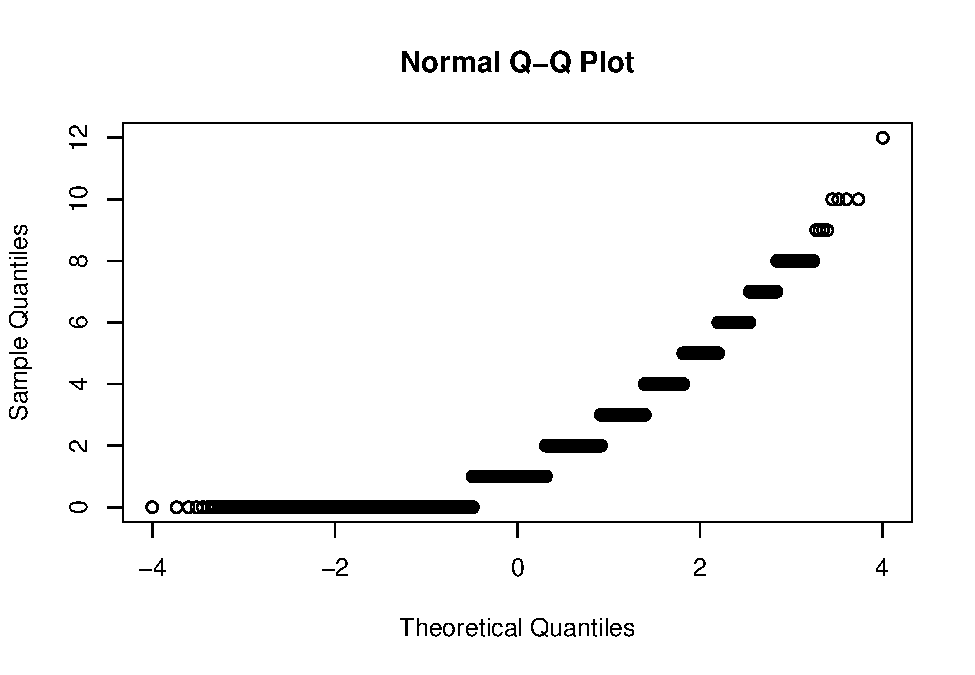
\includegraphics{01-intro_files/figure-latex/unnamed-chunk-6-1.pdf}

Il est très difficile de conclure à partir d'un graphe qqnorm si une variable pourrait effectivement suivre une loi normale. D'ailleur c'est pourquoi il est préférable d'utiliser le test de normalité de Carlos Jarque et Anil K. Bera appelé Jarque--Bera test. Sur R, ce test peut être effectué avec la fonction \texttt{jarque.bera.test()} disponible dans le package \texttt{tseries}.
\(\begin{cases}  H_0: Les\; résidus\; suivent\; une\; loi\; normale\\  H_1: Les \;résidus\; ne\; suivent\; pas\; une\; loi\; normale \end{cases}\)

\begin{Shaded}
\begin{Highlighting}[]
\CommentTok{\#install.packages("tseries")}
\FunctionTok{library}\NormalTok{(tseries)}
\CommentTok{\#\textgreater{} Registered S3 method overwritten by \textquotesingle{}quantmod\textquotesingle{}:}
\CommentTok{\#\textgreater{}   method            from}
\CommentTok{\#\textgreater{}   as.zoo.data.frame zoo}
\FunctionTok{jarque.bera.test}\NormalTok{(SumSINAPS)}
\CommentTok{\#\textgreater{} }
\CommentTok{\#\textgreater{}  Jarque Bera Test}
\CommentTok{\#\textgreater{} }
\CommentTok{\#\textgreater{} data:  SumSINAPS}
\CommentTok{\#\textgreater{} X{-}squared = 8625.6, df = 2, p{-}value \textless{} 2.2e{-}16}
\end{Highlighting}
\end{Shaded}

Le test précédent indique que la \(p\)-\(value\) est inférieure largement à \(0.5\), on rejette alors l'hypothèse \(H_0\) de normalité de \texttt{SumSINAPS} avec un niveau de confiance de \(95%
\)

\hypertarget{cross}{%
\chapter{Cross-references}\label{cross}}

Cross-references make it easier for your readers to find and link to elements in your book.

\hypertarget{chapters-and-sub-chapters}{%
\section{Chapters and sub-chapters}\label{chapters-and-sub-chapters}}

There are two steps to cross-reference any heading:

\begin{enumerate}
\def\labelenumi{\arabic{enumi}.}
\tightlist
\item
  Label the heading: \texttt{\#\ Hello\ world\ \{\#nice-label\}}.

  \begin{itemize}
  \tightlist
  \item
    Leave the label off if you like the automated heading generated based on your heading title: for example, \texttt{\#\ Hello\ world} = \texttt{\#\ Hello\ world\ \{\#hello-world\}}.
  \item
    To label an un-numbered heading, use: \texttt{\#\ Hello\ world\ \{-\#nice-label\}} or \texttt{\{\#\ Hello\ world\ .unnumbered\}}.
  \end{itemize}
\item
  Next, reference the labeled heading anywhere in the text using \texttt{\textbackslash{}@ref(nice-label)}; for example, please see Chapter \ref{cross}.

  \begin{itemize}
  \tightlist
  \item
    If you prefer text as the link instead of a numbered reference use: \protect\hyperlink{cross}{any text you want can go here}.
  \end{itemize}
\end{enumerate}

\hypertarget{captioned-figures-and-tables}{%
\section{Captioned figures and tables}\label{captioned-figures-and-tables}}

Figures and tables \emph{with captions} can also be cross-referenced from elsewhere in your book using \texttt{\textbackslash{}@ref(fig:chunk-label)} and \texttt{\textbackslash{}@ref(tab:chunk-label)}, respectively.

See Figure \ref{fig:nice-fig}.

\begin{Shaded}
\begin{Highlighting}[]
\FunctionTok{par}\NormalTok{(}\AttributeTok{mar =} \FunctionTok{c}\NormalTok{(}\DecValTok{4}\NormalTok{, }\DecValTok{4}\NormalTok{, .}\DecValTok{1}\NormalTok{, .}\DecValTok{1}\NormalTok{))}
\FunctionTok{plot}\NormalTok{(pressure, }\AttributeTok{type =} \StringTok{\textquotesingle{}b\textquotesingle{}}\NormalTok{, }\AttributeTok{pch =} \DecValTok{19}\NormalTok{)}
\end{Highlighting}
\end{Shaded}

\begin{figure}

{\centering 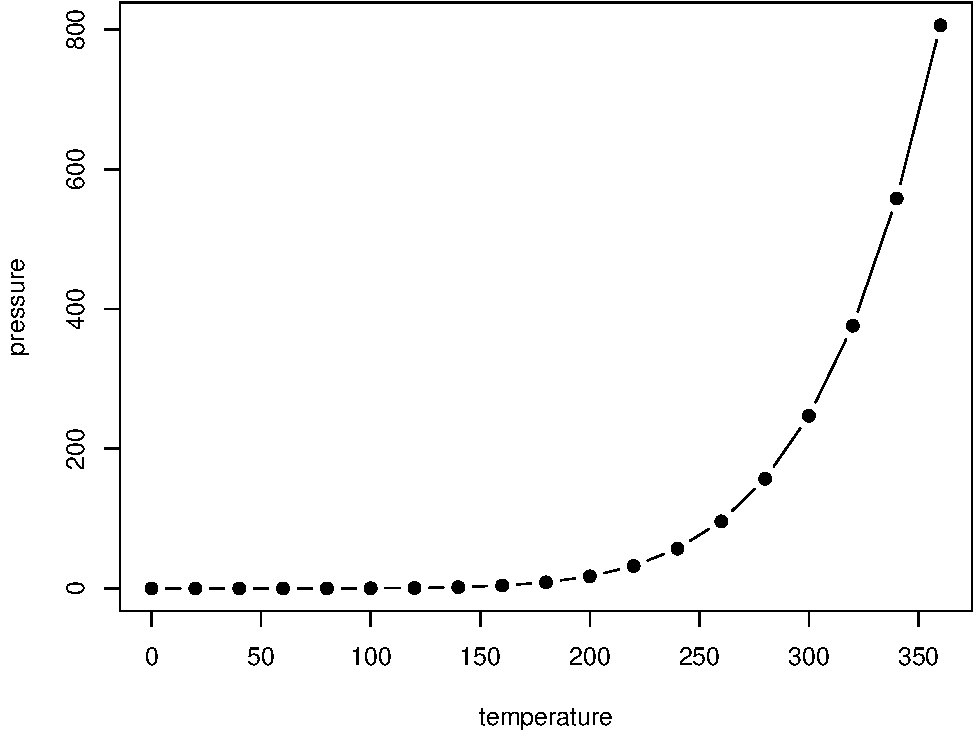
\includegraphics[width=0.8\linewidth]{02-cross-refs_files/figure-latex/nice-fig-1} 

}

\caption{Here is a nice figure!}\label{fig:nice-fig}
\end{figure}

Don't miss Table \ref{tab:nice-tab}.

\begin{Shaded}
\begin{Highlighting}[]
\NormalTok{knitr}\SpecialCharTok{::}\FunctionTok{kable}\NormalTok{(}
  \FunctionTok{head}\NormalTok{(pressure, }\DecValTok{10}\NormalTok{), }\AttributeTok{caption =} \StringTok{\textquotesingle{}Here is a nice table!\textquotesingle{}}\NormalTok{,}
  \AttributeTok{booktabs =} \ConstantTok{TRUE}
\NormalTok{)}
\end{Highlighting}
\end{Shaded}

\begin{table}

\caption{\label{tab:nice-tab}Here is a nice table!}
\centering
\begin{tabular}[t]{rr}
\toprule
temperature & pressure\\
\midrule
0 & 0.0002\\
20 & 0.0012\\
40 & 0.0060\\
60 & 0.0300\\
80 & 0.0900\\
\addlinespace
100 & 0.2700\\
120 & 0.7500\\
140 & 1.8500\\
160 & 4.2000\\
180 & 8.8000\\
\bottomrule
\end{tabular}
\end{table}

\hypertarget{parts}{%
\chapter{Parts}\label{parts}}

You can add parts to organize one or more book chapters together. Parts can be inserted at the top of an .Rmd file, before the first-level chapter heading in that same file.

Add a numbered part: \texttt{\#\ (PART)\ Act\ one\ \{-\}} (followed by \texttt{\#\ A\ chapter})

Add an unnumbered part: \texttt{\#\ (PART\textbackslash{}*)\ Act\ one\ \{-\}} (followed by \texttt{\#\ A\ chapter})

Add an appendix as a special kind of un-numbered part: \texttt{\#\ (APPENDIX)\ Other\ stuff\ \{-\}} (followed by \texttt{\#\ A\ chapter}). Chapters in an appendix are prepended with letters instead of numbers.

\hypertarget{footnotes-and-citations}{%
\chapter{Footnotes and citations}\label{footnotes-and-citations}}

\hypertarget{footnotes}{%
\section{Footnotes}\label{footnotes}}

Footnotes are put inside the square brackets after a caret \texttt{\^{}{[}{]}}. Like this one \footnote{This is a footnote.}.

\hypertarget{citations}{%
\section{Citations}\label{citations}}

Reference items in your bibliography file(s) using \texttt{@key}.

For example, we are using the \textbf{bookdown} package \citep{R-bookdown} (check out the last code chunk in index.Rmd to see how this citation key was added) in this sample book, which was built on top of R Markdown and \textbf{knitr} \citep{xie2015} (this citation was added manually in an external file book.bib).
Note that the \texttt{.bib} files need to be listed in the index.Rmd with the YAML \texttt{bibliography} key.

The \texttt{bs4\_book} theme makes footnotes appear inline when you click on them. In this example book, we added \texttt{csl:\ chicago-fullnote-bibliography.csl} to the \texttt{index.Rmd} YAML, and include the \texttt{.csl} file. To download a new style, we recommend: \url{https://www.zotero.org/styles/}

The RStudio Visual Markdown Editor can also make it easier to insert citations: \url{https://rstudio.github.io/visual-markdown-editing/\#/citations}

\hypertarget{blocks}{%
\chapter{Blocks}\label{blocks}}

\hypertarget{equations}{%
\section{Equations}\label{equations}}

Here is an equation.

\begin{equation} 
  f\left(k\right) = \binom{n}{k} p^k\left(1-p\right)^{n-k}
  \label{eq:binom}
\end{equation}

You may refer to using \texttt{\textbackslash{}@ref(eq:binom)}, like see Equation \eqref{eq:binom}.

\hypertarget{theorems-and-proofs}{%
\section{Theorems and proofs}\label{theorems-and-proofs}}

Labeled theorems can be referenced in text using \texttt{\textbackslash{}@ref(thm:tri)}, for example, check out this smart theorem \ref{thm:tri}.

\begin{theorem}
\protect\hypertarget{thm:tri}{}\label{thm:tri}For a right triangle, if \(c\) denotes the \emph{length} of the hypotenuse
and \(a\) and \(b\) denote the lengths of the \textbf{other} two sides, we have
\[a^2 + b^2 = c^2\]
\end{theorem}

Read more here \url{https://bookdown.org/yihui/bookdown/markdown-extensions-by-bookdown.html}.

\hypertarget{callout-blocks}{%
\section{Callout blocks}\label{callout-blocks}}

The \texttt{bs4\_book} theme also includes special callout blocks, like this \texttt{.rmdnote}.

You can use \textbf{markdown} inside a block.

\begin{Shaded}
\begin{Highlighting}[]
\FunctionTok{head}\NormalTok{(beaver1, }\AttributeTok{n =} \DecValTok{5}\NormalTok{)}
\CommentTok{\#\textgreater{}   day time  temp activ}
\CommentTok{\#\textgreater{} 1 346  840 36.33     0}
\CommentTok{\#\textgreater{} 2 346  850 36.34     0}
\CommentTok{\#\textgreater{} 3 346  900 36.35     0}
\CommentTok{\#\textgreater{} 4 346  910 36.42     0}
\CommentTok{\#\textgreater{} 5 346  920 36.55     0}
\end{Highlighting}
\end{Shaded}

It is up to the user to define the appearance of these blocks for LaTeX output.

You may also use: \texttt{.rmdcaution}, \texttt{.rmdimportant}, \texttt{.rmdtip}, or \texttt{.rmdwarning} as the block name.

The R Markdown Cookbook provides more help on how to use custom blocks to design your own callouts: \url{https://bookdown.org/yihui/rmarkdown-cookbook/custom-blocks.html}

\hypertarget{sharing-your-book}{%
\chapter{Sharing your book}\label{sharing-your-book}}

\hypertarget{publishing}{%
\section{Publishing}\label{publishing}}

HTML books can be published online, see: \url{https://bookdown.org/yihui/bookdown/publishing.html}

\hypertarget{pages}{%
\section{404 pages}\label{pages}}

By default, users will be directed to a 404 page if they try to access a webpage that cannot be found. If you'd like to customize your 404 page instead of using the default, you may add either a \texttt{\_404.Rmd} or \texttt{\_404.md} file to your project root and use code and/or Markdown syntax.

\hypertarget{metadata-for-sharing}{%
\section{Metadata for sharing}\label{metadata-for-sharing}}

Bookdown HTML books will provide HTML metadata for social sharing on platforms like Twitter, Facebook, and LinkedIn, using information you provide in the \texttt{index.Rmd} YAML. To setup, set the \texttt{url} for your book and the path to your \texttt{cover-image} file. Your book's \texttt{title} and \texttt{description} are also used.

This \texttt{bs4\_book} provides enhanced metadata for social sharing, so that each chapter shared will have a unique description, auto-generated based on the content.

Specify your book's source repository on GitHub as the \texttt{repo} in the \texttt{\_output.yml} file, which allows users to view each chapter's source file or suggest an edit. Read more about the features of this output format here:

\url{https://pkgs.rstudio.com/bookdown/reference/bs4_book.html}

Or use:

\begin{Shaded}
\begin{Highlighting}[]
\NormalTok{?bookdown}\SpecialCharTok{::}\NormalTok{bs4\_book}
\end{Highlighting}
\end{Shaded}


  \bibliography{book.bib,packages.bib}

\end{document}
